\documentclass[12pt]{article}
\usepackage[top=0.5in, bottom=0.8in, left=0.5in, right=0.5in]{geometry}

\usepackage{amsmath,amssymb,amsfonts,amsthm}
\usepackage[english]{babel}
\usepackage[T1]{fontenc}
\usepackage{bm}
\usepackage{verbatim}
\usepackage[all]{xy}
\usepackage[pdftex]{hyperref}
\usepackage{graphicx}
\graphicspath{ {./} }
\hypersetup{colorlinks=false, linkcolor=blue, pdffitwindow=true, pdftitle={Oscillation}}

\title{Oscillation Detection}
\author{Wei Cui}
\begin{document}
\maketitle
\section{Oscillation Detection}
In the topic of pollen tube growth, there are three kinds of signal which we can care about. The first is from F-actin which we still can not measure for now. The others are from ROP1 and Calclum which we can measure and they should be oscillation theoretically. Unfortunately, the signal is always not good enough. One of the best is shown in the top plot of \ref{fig:first}. So the first task is to detect oscillation from the raw signal. \\

Convolution is a useful tool to this problem. There are some similar (but different) definations of convolution. We will use the following two of them. \\

Denote the original data list as $\left\{X_{1}, X_{2}, \ldots, X_{n}\right\}$. \\

Denote the center symmetric transform of $X_{n}$ as $\left\{Y_{1}, Y_{2}, \ldots, Y_{2n-1}\right\}$ where $Y_{i} = X_{i}$ when $i = 1, 2, \ldots, n$, $Y_{i} = X_{2n-i}$ when $i = n + 1, n + 2, \ldots, 2n - 1$. \\

Denote the right expand list as $\left\{Z_{1}, Z_{2}, \ldots, Z_{2n-1}\right\}$, where $Z_{i} = X_{i}$ when $i = 1, 2, \ldots, n$, $Z_{i} = 0$ when $i = n + 1, n + 2, \ldots, 2n - 1$. \\

The first defination is about $X$ and $Y$. The convolution $\left\{C_{1}, C_{2}, \ldots, C_{n}\right\}$ will be: 

\begin{equation}
C_{i} = \sum_{j=0}^{n-1}X_{i+j}Y_{i+j}
\end{equation}

The second defination is about $X$ and $Z$. The convolution $\left\{C_{1}, C_{2}, \ldots, C_{n}\right\}$ will be: 
\begin{equation}
C_{i} = \sum_{j=0}^{n-1}X_{i+j}Z_{i+j}
\end{equation}

The result of these two definations (to the dataset mentioned above) is almost the same as the plots shown in \ref{fig:first}. Then we can determine a threshold of peak values and do clustering to get period of the data. \\

Tt seems that the problem is solved but actually it is not. There are some other kind of data, for example the top plot of \ref{fig:second}. The data has some trend so the pure convolution method is not efficient here. We have to eliminate the effect of trend. One method is linear regression but we can not always suppose the trend is linear. \\

Here we apply empirical mode decomposition (EMD) from Hilbert-Huang transform (HHT). HHT is used to get instant frequency of data and EMD will decompose the original data to a series of intrinsic mode function (IMF) and a trend function which we desire to get. We use this trend function to modify the original data and the result is in \ref{fig:first} and \ref{fig:second}. \\ 

\begin{figure}[h]
\caption{The result of the first dataset. Top: standarized data. Middle: result of defination one with modification. Bottom: result of defination two with modification.}
\label{fig:first}
\centering
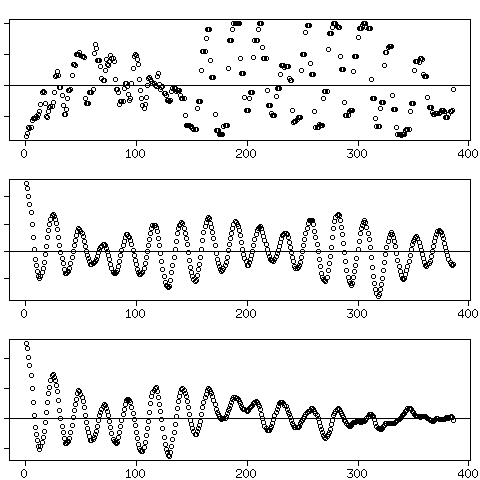
\includegraphics{012}
\end{figure}

\begin{figure}[h]
\caption{The result of the second dataset. Top: standarized data. Middle: result of defination one with modification. Bottom: result of defination two with modification.}
\label{fig:second}
\centering
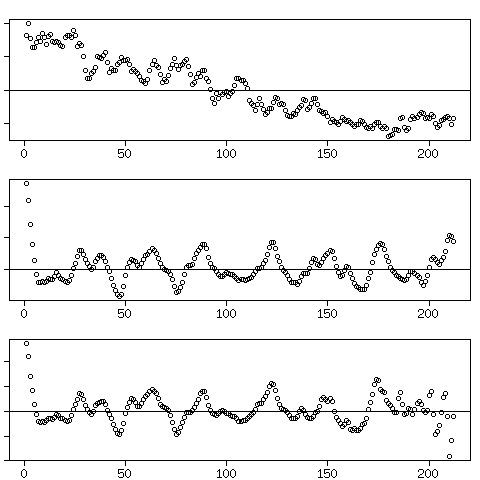
\includegraphics{002}
\end{figure}

Positive: \\

1. The method is very simple. \\

2. It is actually very fast since the convolution manipulation can be done by fast Fourier transform (But EMD will take some time). \\

3. The result is acceptable. \\ \\

Negative: \\

1. The result depends on the head part of original data which means if only some other part of the data is oscillation then the method will be not so efficient. \\

2. The tail part of the result is not very confidential since there are not enough data point in the tail. \\

3. There is no universal method to determine the threshold value. \\ \\

\section{Growth model include ROP1 and Calcium}

In the previous model, only the signal of ROP1 is considered. The final target is to cover the signal of ROP1, F-actin and Calclum. Because the F-actin is not measurable for now, Nan Luo suggest a model include the signal of ROP1 and Calcium as follows.

\begin{equation}
  \begin{array}{rcl}
    \frac{\partial{}R(t)}{\partial{}t} & = & k_{pf}(R_{total} - R(t)) - k_{nf}C(t)R(t) \\
    & & \\
    \frac{\partial{}C(t)}{\partial{}t} & = & k_{a}(R(t - \tau) + C_{0}) - k_{d}C(t)
  \end{array}
\end{equation}

Four assumptions: \\

1. The time interval between any two continuous measurements is very small; \\

2. The time interval between any two continuous measurements is constant. \\

3. The parameter $\tau$ is non-negative integer.\\

4. The upper bound of period length $L$ can be estimated from data. (With the result of Oscillation Detection part, this assumption can be satisfied.)\\

The first assumption allows us to replace differential equation with difference equation. The parameter $\tau$ can be estimated with assumption 2 and 3. The parameter space of $\tau$ is limited with assumption 3 and 4. \\
\\

The method: \\

1. let $t = 0, 1, 2, \ldots , N$ as the sampling time. \\

2. To $t = 1, 2, \ldots , N - 1$, replace $\frac{\partial{}R(t)}{\partial{}t}$ with $\frac{R(t + 1) - R(t - 1)}{2}$, replace $\frac{\partial{}C(t)}{\partial{}t}$ with $\frac{C(t + 1) - C(t - 1)}{2}$. Replace $k_{pf}R_{total}$ with $kR$, replace $k_{a}C_{0}$ with $kC$. Then the formula becomes:

\begin{equation}
  \begin{array}{rcl}
    \frac{R(t + 1) - R(t - 1)}{2} & = & kR - k_{pf}R(t) - k_{nf}C(t)R(t) \\
    & & \\
    \frac{C(t + 1) - C(t - 1)}{2} & = & k_{a}R(t - \tau) + kC - k_{d}C(t)
  \end{array}
\end{equation}

3. Estimate $kR, k_{pf}, k_{nf}$ by ordinary least squares (OLS) or generalized least squares (GLS). \\ 

4. Let $\tau = 0$. Then we can get OLS estimation or GLS estimation of $kC, k_{a}, k_{d}$. \\

5. Let $\tau = \tau + 1$ and return to step 4 until $\tau = L$. \\

6. Choose the best $\tau$ from $L + 1$ estimations. \\ \\

Positive: \\

1. The method is simple enouph. \\

2. The method can estimate all the parameters. \\ \\

Negative: \\

1. The method will import new computational errors. \\ \\

An alternative method is to eliminate $C(t)$ from the equation array to get an ODE of $R(t)$ and then solve this ODE. But it will be difficult to estimate all the parameters. 

\end{document}
